\documentclass[11pt, a4paper]{article}

% Basic packages
\usepackage{amsmath,amssymb,amsfonts}
\usepackage{bm,ltablex,microtype}
\usepackage{graphicx}
\usepackage[utf8]{inputenc}
\usepackage{parskip}
\usepackage[section]{placeins}
\usepackage[capitalise, noabbrev]{cleveref}
\usepackage{fancyvrb}
\usepackage{csvsimple}
\usepackage{booktabs}
\usepackage[margin=3cm]{geometry}
\usepackage[table,xcdraw]{xcolor}
\usepackage{tikz}
\usetikzlibrary{math,calc,positioning}

\usepackage{todonotes}

% Set up fonts
% \usepackage{fontspec}
% \usepackage{unicode-math}
% \setmainfont{STIX Two Text}
% \setmathfont{STIX Two Math}

\title{FYS-STK4155 - Project1}
\author{Gard, Are, David Andreas Bordvik}
\date{\today}

\begin{document}

\maketitle
\section*{Theory}
MSE value between $\boldsymbol{y}$ and $\boldsymbol{\hat y}$ is defined as;
\begin{equation}
    MSE(\boldsymbol{y},\boldsymbol{\tilde{y}}) = \frac{1}{n}
    \sum_{i=0}^{n-1}(y_i-\tilde{y}_i)^2
\end{equation}

The $R^2$ value between $\boldsymbol{y}$ and $\boldsymbol{\hat y}$ is defined as;
\begin{equation}
    R^2(\boldsymbol{y}, \tilde{\boldsymbol{y}}) = 1 - \frac{\sum_{i=0}^{n - 1} (y_i - \tilde{y}_i)^2}{\sum_{i=0}^{n - 1} (y_i - \bar{y})^2}
\end{equation}

The mean value of $\boldsymbol{y}$ is defined as;
\begin{equation}
    \bar{y} =  \frac{1}{n} \sum_{i=0}^{n - 1} y_i
\end{equation}

The variance of $\boldsymbol{y}$ is defined as;
\begin{equation}
    \mathrm{var}[\boldsymbol{x}]=\frac{1}{n}\sum_{i=0}^{n-1}(x_i- \overline{x})^2=\mathbb{E}\left[(\bm{y}-\bm{\tilde{y}})^2\right]
\end{equation}



\section*{Exercise 1}
\begin{figure}
  \centering
  \includegraphics{figures/franke_function_preview.pdf}
  \caption{?}
  \label{fig: ?}
\end{figure}

\begin{figure}
  \centering
  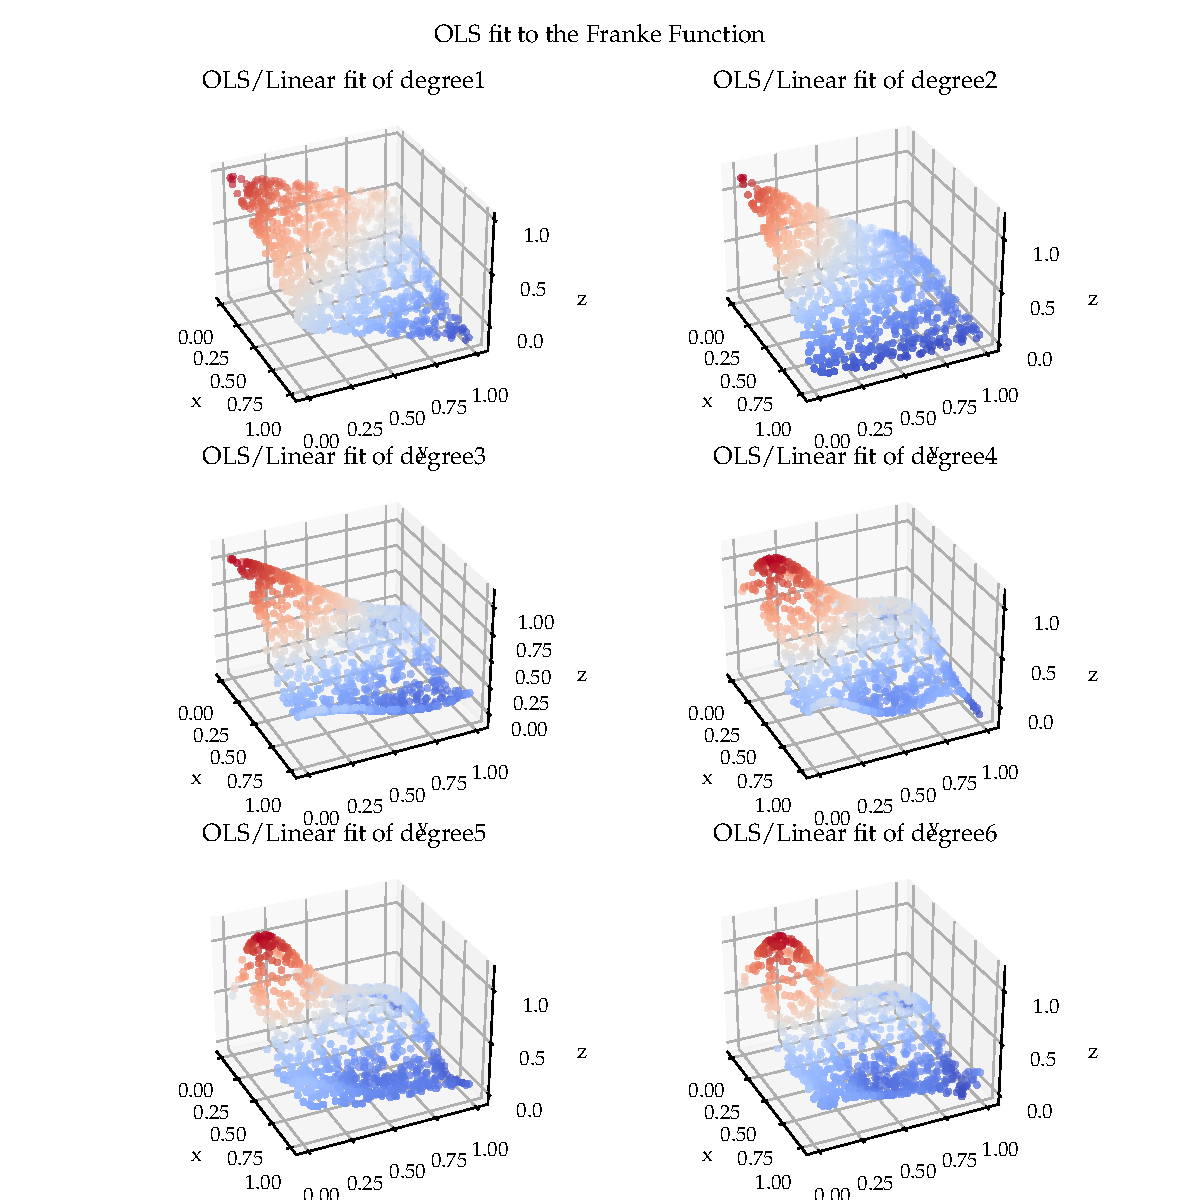
\includegraphics[scale=0.85]{figures/franke_function_OLS_fit.pdf}
  \caption{?}
  \label{fig: ?}
\end{figure}

\begin{figure}
  \centering
  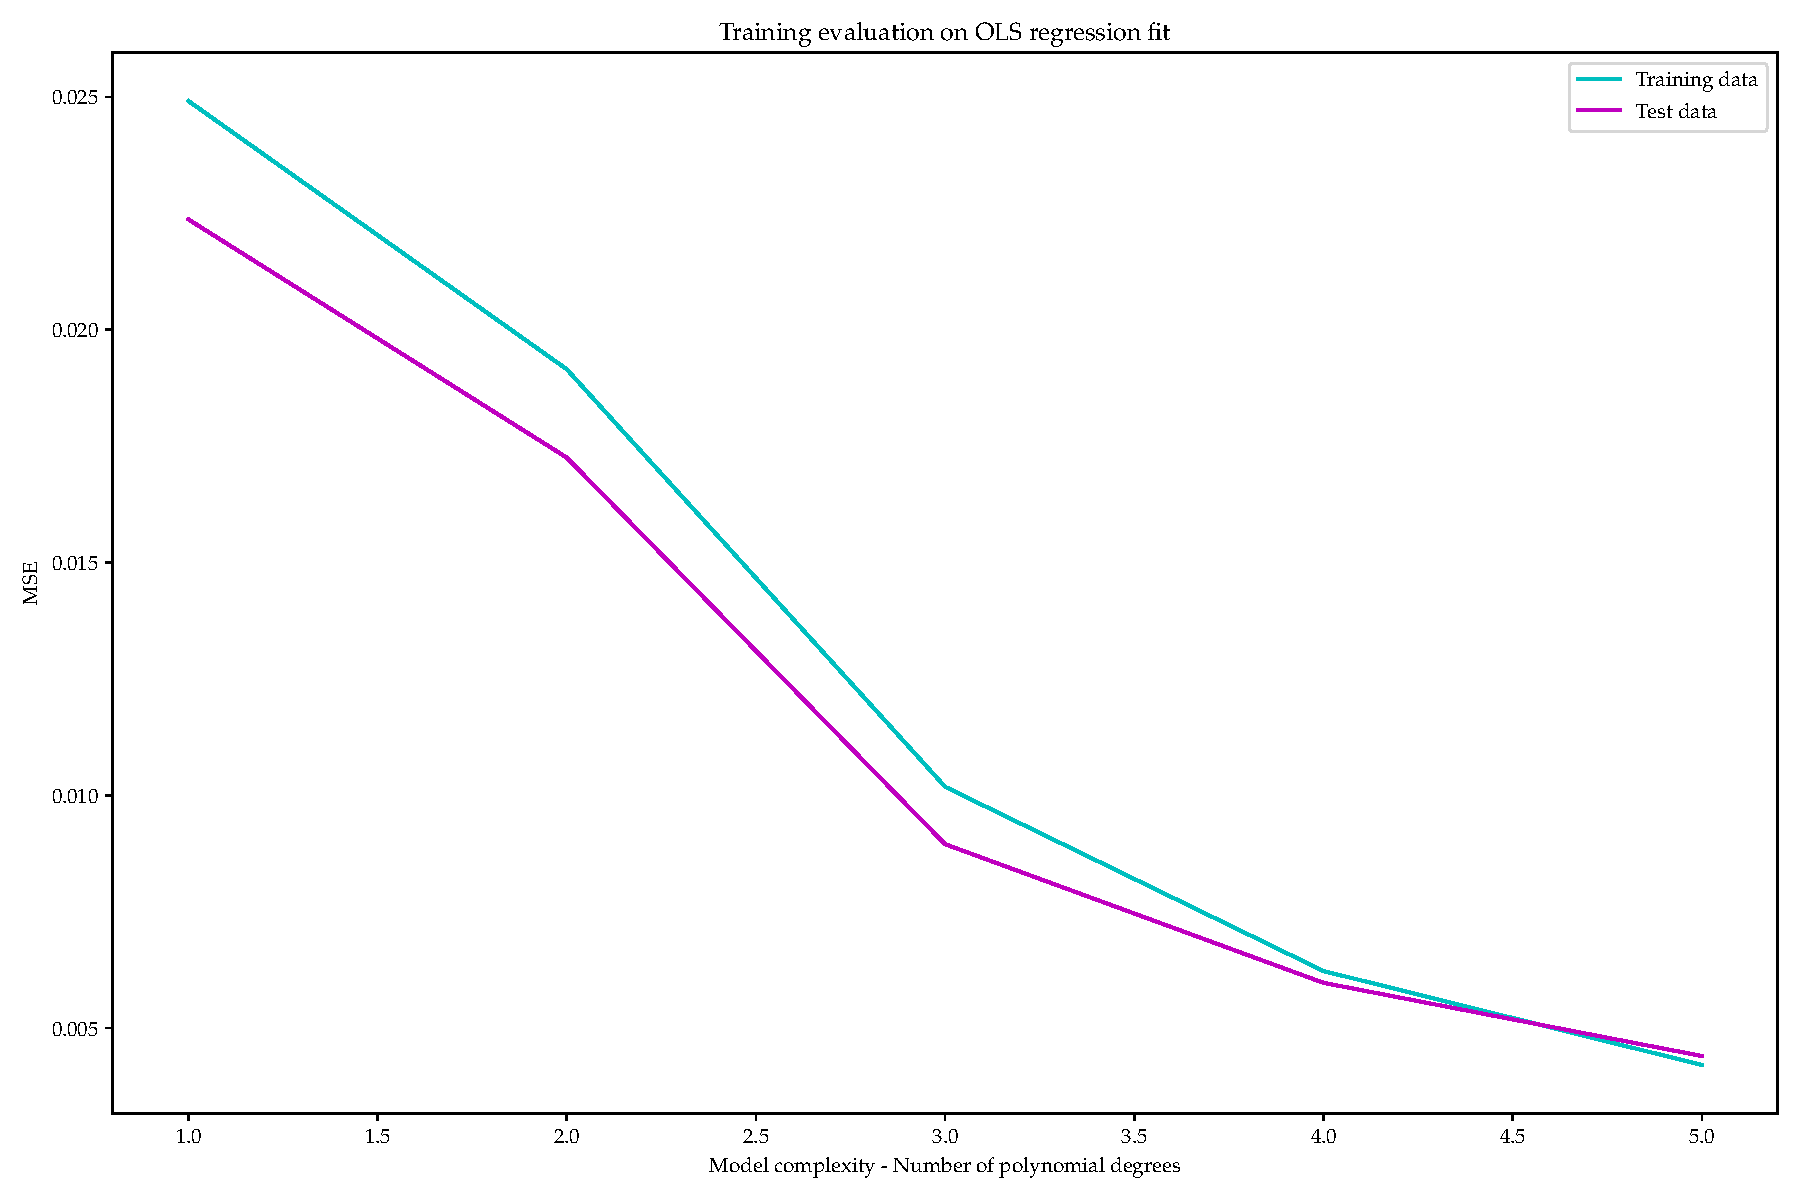
\includegraphics[scale=0.45]{figures/franke_function_OLS_evaluate_fit.pdf}
  \caption{?}
  \label{fig: ?}
\end{figure}

\begin{figure}
  \centering
  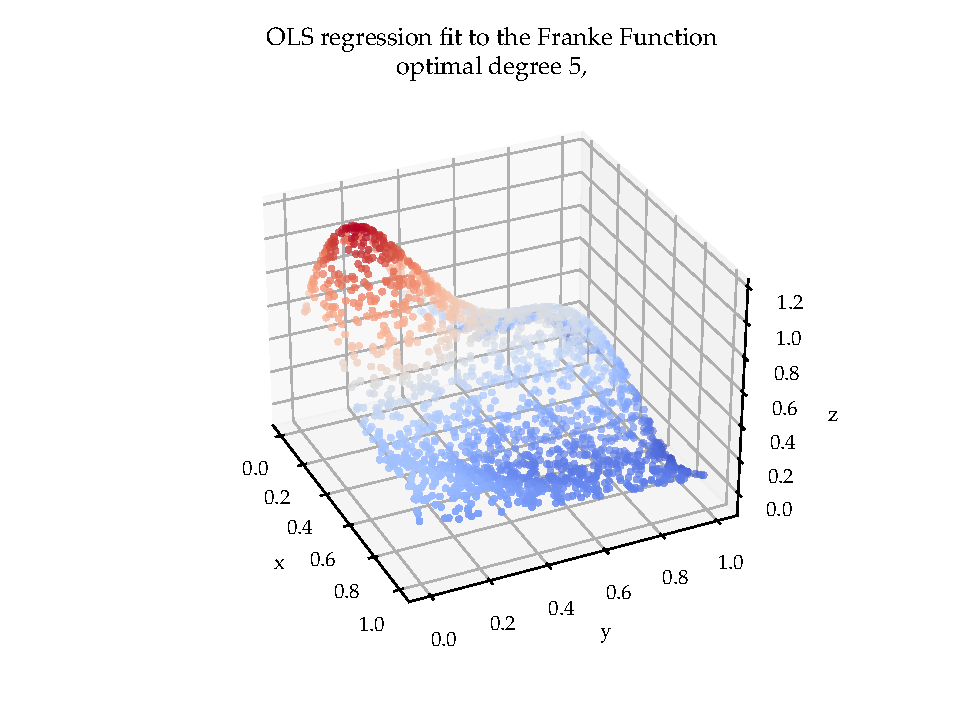
\includegraphics[scale=0.85]{figures/franke_function_OLS_best_fit.pdf}
  \caption{?}
  \label{fig: ?}
\end{figure}


\section*{Exercise 2}
Moving on to the bias-variance trade-off analysis, we start off by showing that 

\[
  C(\bm{X},\bm{\beta}) =\frac{1}{n}\sum_{i=0}^{n-1}(y_i-\tilde{y}_i)^2=\mathbb{E}\left[(\bm{y}-\bm{\tilde{y}})^2\right]
\]

Can be rewritten as

\[
\mathbb{E}\left[(\bm{y}-\bm{\tilde{y}})^2\right]=\frac{1}{n}\sum_i(f_i-\mathbb{E}\left[\bm{\tilde{y}}\right])^2+\frac{1}{n}\sum_i(\tilde{y}_i-\mathbb{E}\left[\bm{\tilde{y}}\right])^2+\sigma^2.
\]

where the terms are respectively $(\text{bias})^2$, variance and noise. For simplicity, assume that we have a dataset where the data is generated from a noisy model

\[\bm{y} = f(\bm{x}) + \bm{\epsilon}\]

Furthermore, we will assume that the residuals $\epsilon$ are independant and normally distributed $\epsilon \sim \mathcal{N}(0, \sigma^2)$. Finally, $\bm{\tilde{y}} = \bm{X}\bm{\beta}$ is our approximation to the functions $f$. Start off by adding and subtracting $\mathbb{E}\left[\bm{\tilde{y}}\right]$ inside the expectation value.

\[
  \mathbb{E}\left[(\bm{y}-\bm{\tilde{y}})^2\right] 
  = \mathbb{E}\left[(\bm{y}-\bm{\tilde{y}} + \mathbb{E}\left[\bm{\tilde{y}}\right] - \mathbb{E}\left[\bm{\tilde{y}}\right])^2\right] 
\]
\[
  = \mathbb{E}\left[((\bm{y} - \mathbb{E}\left[\bm{\tilde{y}}\right]) - (\bm{\tilde{y}} - \mathbb{E}\left[\bm{\tilde{y}}\right]))^2\right]
\]
By using the fact that $\bm{y} = f(\bm{x}) + \bm{\epsilon}$
we can rewrite this as
\[
  = \mathbb{E}\left[((f(\bm{x}) - \mathbb{E}\left[\bm{\tilde{y}}\right]) - (\bm{\tilde{y}} - \mathbb{E}\left[\bm{\tilde{y}}\right]) + \epsilon)^2\right]
\]
Computing the square inside the expectation value gives us
\[
  = \mathbb{E}\left[(f(\bm{x}) - \mathbb{E}\left[\bm{\tilde{y}}\right])^2 + (\bm{\tilde{y}} - \mathbb{E}\left[\bm{\tilde{y}}\right])^2 + \epsilon^2 \right]\]
  \[+ 2\left(\mathbb{E}\left[\epsilon(f(\bm{x}) - \mathbb{E}\left[\bm{\tilde{y}}\right])\right]- \mathbb{E}\left[\epsilon(\bm{\tilde{y}} - \mathbb{E}\left[\bm{\tilde{y}}\right])\right] - \mathbb{E}\left[(f(\bm{x}) - \mathbb{E}\left[\bm{\tilde{y}}\right])(\bm{\tilde{y}} - \mathbb{E}\left[\bm{\tilde{y}}\right])\right]\right)
\]
Moreover, as $\epsilon$ are independant variables, the expectation value involving them as a product can be written as a product of expectation values. Knowing that $\mathbb{E}\left[\epsilon\right] = 0$, the third and second to last term is equal to zero. Also, knowing that $\mathbb{E}\left[\bm{\tilde{y}}\right] = \bm{\tilde{y}}$, the last t

\begin{equation}\label{eq:varbi}
  = \mathbb{E}\left[(f(\bm{x}) - \mathbb{E}\left[\bm{\tilde{y}}\right])^2\right] + \mathbb{E}\left[(\bm{\tilde{y}} - \mathbb{E}\left[\bm{\tilde{y}}\right])^2\right] + \mathbb{E}\left[\epsilon^2 \right]
\end{equation}
The first term in (\ref{eq:varbi}) can be discretized as
\[
  \mathbb{E}\left[(f(\bm{x}) - \mathbb{E}\left[\bm{\tilde{y}}\right])^2\right] = \frac{1}{n}\sum_i(f_i - \mathbb{E}\left[\bm{\tilde{y}}\right])^2
\]
Which is the bias squared as we were to show.

The second term in (\ref{eq:varbi}) is also discretized, yielding
\[
  \mathbb{E}\left[(\bm{\tilde{y}} - \mathbb{E}\left[\bm{\tilde{y}}\right])^2\right] = \frac{1}{n}\sum_i(\bm{\tilde{y}} - \mathbb{E}\left[\bm{\tilde{y}}\right])^2
\]
Which takes form of the variance, as was set out to show.

Finally, it can be shown that $\text{var}(\bm{y}) = \text{var}(f + \epsilon) = \mathbb{E}\left[(f + \epsilon)^2\right] - (\mathbb{E}\left[(f + \epsilon)\right])^2$ = $\mathbb{E}\left[\epsilon^2\right]$ As such, we can use that \[
  \text{var}(y) = \sigma^2 = \mathbb{E}\left[\epsilon^2\right]
\]
to see that the final term in (\ref{eq:varbi}) is equal to the noise. Thus we have shown that 
\[
\mathbb{E}\left[(\bm{y}-\bm{\tilde{y}})^2\right] = \mathbb{E}\left[(f(\bm{x}) - \mathbb{E}\left[\bm{\tilde{y}}\right])^2\right] + \mathbb{E}\left[(\bm{\tilde{y}} - \mathbb{E}\left[\bm{\tilde{y}}\right])^2\right] + \mathbb{E}\left[\epsilon^2 \right]
\]
\[
=\frac{1}{n}\sum_i(f_i-\mathbb{E}\left[\bm{\tilde{y}}\right])^2+\frac{1}{n}\sum_i(\tilde{y}_i-\mathbb{E}\left[\bm{\tilde{y}}\right])^2+\sigma^2.
\]

\begin{figure}
  \centering
  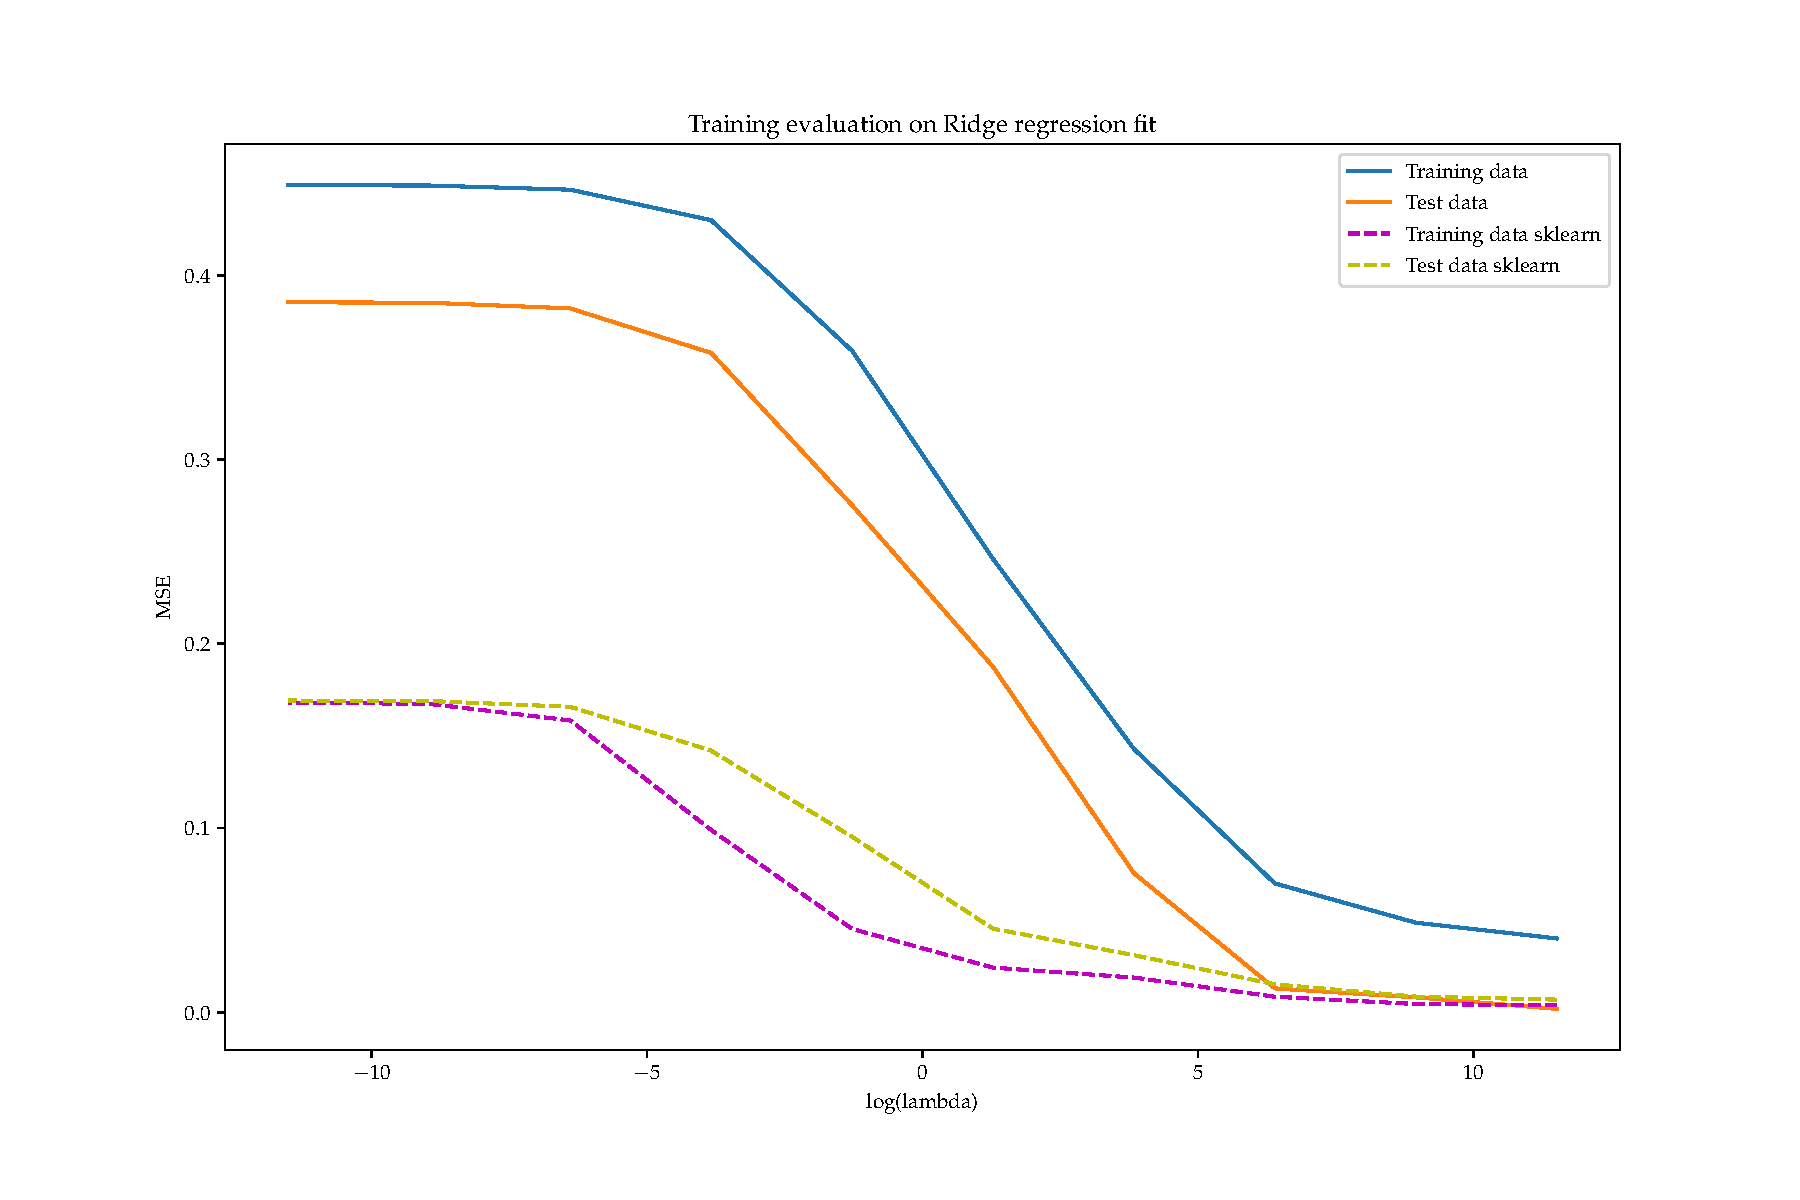
\includegraphics[scale=0.45]{figures/franke_function_Ridge_evaluate_fit.pdf}
  \caption{The best fit using Ridge}
  \label{fig: Ridge_best_fit}
\end{figure}

\begin{figure}
  \centering
  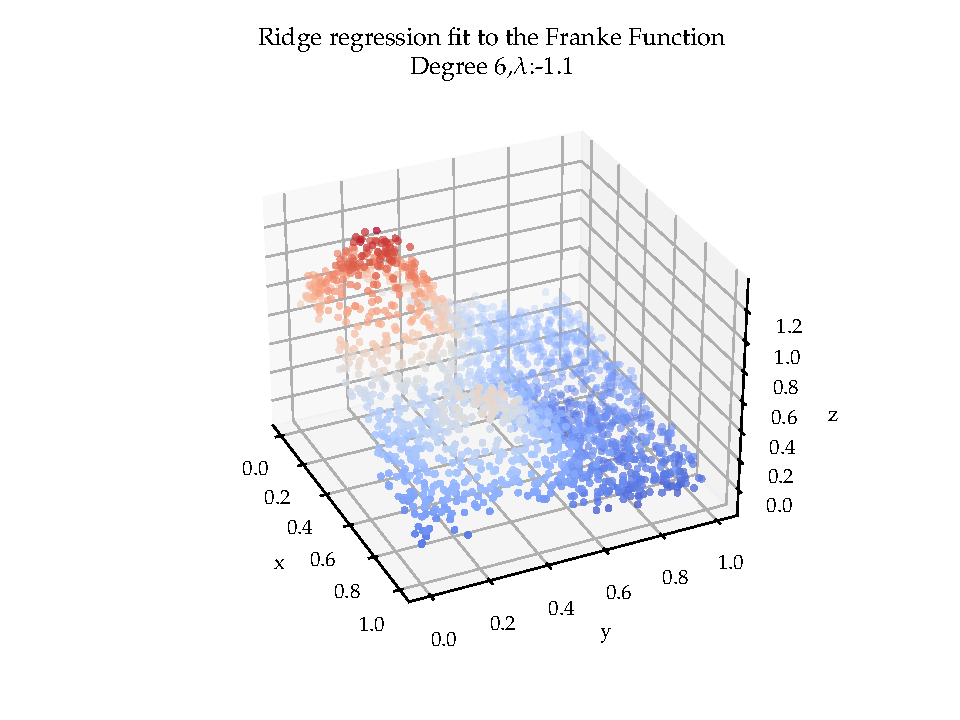
\includegraphics[scale=0.85]{figures/franke_function_Ridge_best_fit.pdf}
  \caption{The best fit using Ridge}
  \label{fig: Ridge_best_fit}
\end{figure}

\begin{center}
  \csvautobooktabular{data/report_data/redge_reg_lambda_-1.1.csv}
  \label{data: Ridge_best_fit}
\end{center}



\newpage
\newpage


\bibliography{bibliography}
\bibliographystyle{ieeetr}



\end{document}


% Local Variables:
% TeX-engine: xetex
% End:
